\documentclass{beamer}
\usepackage[utf8]{inputenc}
\usepackage[T1]{fontenc}
\usepackage[english]{babel}
\usepackage{hyperref}
\usepackage{outlines}
\usepackage{graphicx}
\usepackage{algorithm}
\usepackage{algorithmic}
\usepackage{amsmath,amssymb}
\usepackage{moresize}
\usepackage{tikz}
\usetikzlibrary{positioning,arrows.meta}
\usetikzlibrary{overlay-beamer-styles}
\usepackage{microtype}
\usepackage[
  backend=biber,
  style=alphabetic,
]{biblatex}
\usepackage{latexsym,multicol,booktabs,calligra}
\usepackage{listings,stackengine}
\usepackage[table,dvipsnames]{xcolor}
\usepackage{cancel}
\renewcommand{\figurename}{Figure}
\renewcommand{\algorithmname}{Algorithm}

\usepackage{SHU}
\setbeamersize{text margin left=7mm, text margin right=7mm}
\definecolor{deepblue}{rgb}{0,0,0.5}
\definecolor{deepred}{rgb}{0.6,0,0}
\definecolor{deepgreen}{rgb}{0,0.5,0}
\definecolor{halfgray}{gray}{0.55}
\definecolor{nus-orange}{RGB}{239,124,0}
\definecolor{nus-blue}{RGB}{0,61,124}

\lstset{
  language=SQL,
  basicstyle=\ttfamily\tiny,
  keywordstyle=\bfseries\color{nus-blue},
  emphstyle=\ttfamily\color{nus-blue},
  stringstyle=\color{deepgreen},
  numbers=left,
  numberstyle=\scriptsize\color{halfgray},
  rulesepcolor=\color{nus-orange},
  frame=shadowbox,
  showstringspaces=false,
  breaklines=true,
  breakatwhitespace=true,
  keepspaces=true,
  columns=flexible,
  upquote=true
}


\author{\href{https://pratik2358.github.io/}{Pratik Karmakar}}
\title{IT5008: Tutorial — BEFORE/AFTER Triggers \& Cursors in PostgreSQL}
\institute{
  School of Computing,\\
  National University of Singapore
}
\date{AY25/26 S1}

\begin{document}

% Title
\begin{frame}
  \titlepage
\end{frame}

% Agenda
\begin{frame}{Agenda}
\begin{outline}
  \1 Database context (borrowers, copies, loans)
  \1 Trigger timing: BEFORE vs AFTER
    \2 Local (row-level) constraint via BEFORE
    \2 Global invariant via AFTER (+rollback on exception)
  \1 Step-by-step demo timeline
  \1 Cursors: what/why/how, with example
  \1 Takeaways \& pitfalls
\end{outline}
\end{frame}

% Schema recap (minimal)
\begin{frame}{Database Context (Minimal)}
\begin{itemize}
  \item \texttt{copy(owner, book, copy)}: physical copies of books (book \(\approx\) ISBN13)
  \item \texttt{loan(borrower, owner, book, copy, borrowed, returned)}
  \begin{itemize}
    \item Active loan: \texttt{returned IS NULL}
  \end{itemize}
\end{itemize}
\begin{block}{Goal}
Enforce: a borrower may have at most \(\mathbf{3}\) active loans.
\end{block}
\end{frame}

% BEFORE trigger example
\begin{frame}[fragile]{BEFORE Trigger (Local Loan Limit)}
\textbf{Intent:} Prevent inserting a loan row if the borrower already has 3 active loans.\\[2mm]
\begin{lstlisting}
CREATE OR REPLACE FUNCTION check_local_loan_limit()
RETURNS TRIGGER AS $$
DECLARE active_loan_count INT;
BEGIN
  SELECT COUNT(*) INTO active_loan_count
  FROM loan
  WHERE borrower = NEW.borrower
    AND returned IS NULL;

  IF active_loan_count >= 3 THEN
    RAISE NOTICE 'Loan limit reached for %', NEW.borrower;
    RETURN NULL;             -- Block the insert
  END IF;

  RETURN NEW;                -- Allow insert as-is (or modified)
END;
$$ LANGUAGE plpgsql;

CREATE TRIGGER enforce_local_limit
BEFORE INSERT ON loan
FOR EACH ROW
EXECUTE FUNCTION check_local_loan_limit();
\end{lstlisting}
\end{frame}

\begin{frame}{BEFORE Trigger: Behaviour}
\begin{itemize}
  \item Fires \textbf{before} the row is written.
  \item \texttt{RETURN NULL} \(\Rightarrow\) cancels the event (no row added, no rollback needed).
  \item \texttt{RETURN NEW} \(\Rightarrow\) proceed, possibly with edited values.
  \item Perfect for \textbf{local, per-row} constraints.
\end{itemize}
\begin{block}{Example}
\texttt{INSERT INTO loan(...)} \(\rightarrow\) \texttt{NOTICE: Loan limit reached for alice@example.com} \(\rightarrow\) blocked.
\end{block}
\end{frame}

% AFTER trigger example
\begin{frame}[fragile]{AFTER Trigger (Global Loan Limit)}
\textbf{Intent:} Ensure \emph{no} borrower in the whole system exceeds 3 active loans (detect after write).\\[2mm]
\tiny
\begin{lstlisting}
CREATE OR REPLACE FUNCTION check_global_loan_limit()
RETURNS TRIGGER AS $$
DECLARE violator RECORD;
BEGIN
  SELECT borrower INTO violator
  FROM loan
  WHERE returned IS NULL
  GROUP BY borrower
  HAVING COUNT(*) > 3;

  IF violator IS NOT NULL THEN
    RAISE EXCEPTION 'Borrower % exceeds global limit', violator.borrower;
  END IF;

  RETURN NEW;  -- Required, though AFTER cannot change the row
END;
$$ LANGUAGE plpgsql;

CREATE TRIGGER enforce_global_limit
AFTER INSERT OR UPDATE ON loan
FOR EACH ROW
EXECUTE FUNCTION check_global_loan_limit();
\end{lstlisting}
\end{frame}

\begin{frame}{AFTER Trigger: Behaviour \& Rollback}
\begin{itemize}
  \item Fires \textbf{after} the row is written (but before commit).
  \item If it \texttt{RAISE EXCEPTION}:
    \begin{itemize}
      \item PostgreSQL \textbf{aborts the transaction} automatically.
      \item All changes in the current transaction are \textbf{rolled back}.
    \end{itemize}
  \item Ideal for \textbf{global invariants}, auditing, notifications.
\end{itemize}
\begin{block}{Effect}
Insert appears to succeed \(\rightarrow\) AFTER trigger runs \(\rightarrow\) exception \(\rightarrow\) transaction rolled back \(\Rightarrow\) no net change.
\end{block}
\end{frame}

%-------------------------------------------
\begin{frame}{Execution Timeline (INSERT) — \textbf{BEFORE} Trigger}
\centering
\scalebox{0.85}{%
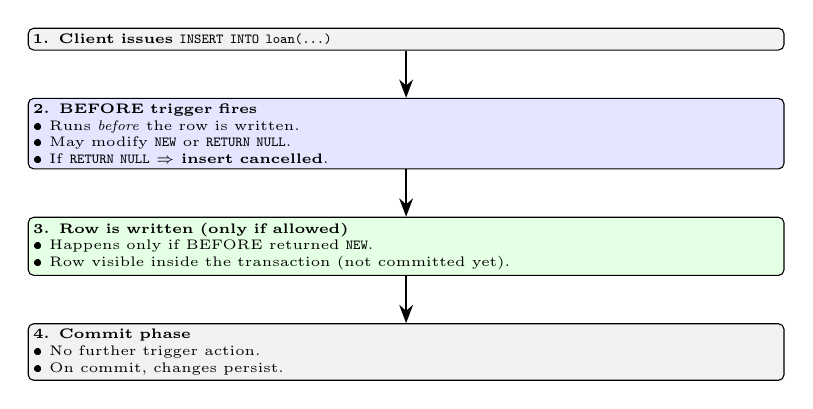
\begin{tikzpicture}[
  >=Stealth,
  node distance=6mm,
  box/.style={
    rectangle, draw, rounded corners=2pt, align=left,
    inner sep=2pt, text width=.78\linewidth, font=\tiny
  },
  arrow/.style={->, thick}
]
\node (s1) [box, fill=gray!10]
  {\textbf{1. Client issues} \texttt{INSERT INTO loan(...)}};

\node (s2) [box, fill=blue!10, below=of s1]
  {\textbf{2. BEFORE trigger fires}\\
   • Runs \emph{before} the row is written.\\
   • May modify \texttt{NEW} or \texttt{RETURN NULL}.\\
   • If \texttt{RETURN NULL} $\Rightarrow$ \textbf{insert cancelled}.};

\node (s3) [box, fill=green!10, below=of s2]
  {\textbf{3. Row is written (only if allowed)}\\
   • Happens only if BEFORE returned \texttt{NEW}.\\
   • Row visible inside the transaction (not committed yet).};

\node (s4) [box, fill=gray!10, below=of s3]
  {\textbf{4. Commit phase}\\
   • No further trigger action.\\
   • On commit, changes persist.};

\draw[arrow] (s1) -- (s2);
\draw[arrow] (s2) -- (s3);
\draw[arrow] (s3) -- (s4);
\end{tikzpicture}
}
\vspace{1mm}

{\scriptsize\textcolor{nus-blue}{\textbf{Summary:}} BEFORE can directly \textbf{block} the insert by returning \texttt{NULL}; otherwise the row proceeds to insert and commit.}
\end{frame}

\begin{frame}{Execution Timeline (INSERT) — \textbf{AFTER} Trigger}
\centering
\scalebox{0.85}{%
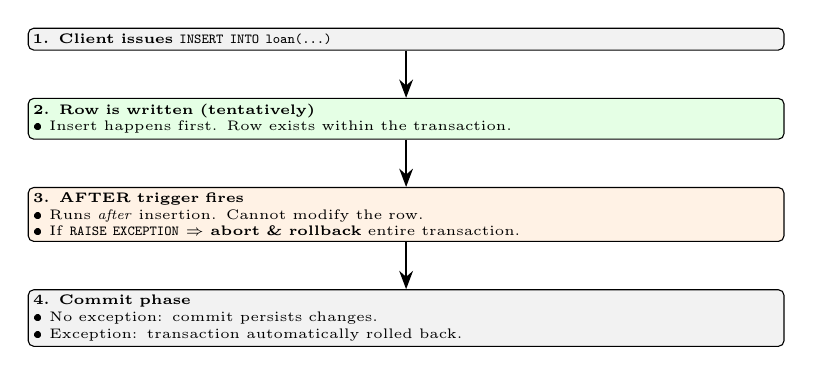
\begin{tikzpicture}[
  >=Stealth,
  node distance=6mm,
  box/.style={
    rectangle, draw, rounded corners=2pt, align=left,
    inner sep=2pt, text width=.78\linewidth, font=\tiny
  },
  arrow/.style={->, thick}
]
\node (a1) [box, fill=gray!10]
  {\textbf{1. Client issues} \texttt{INSERT INTO loan(...)}};

\node (a2) [box, fill=green!10, below=of a1]
  {\textbf{2. Row is written (tentatively)}\\
   • Insert happens first. Row exists within the transaction.};

\node (a3) [box, fill=orange!10, below=of a2]
  {\textbf{3. AFTER trigger fires}\\
   • Runs \emph{after} insertion. Cannot modify the row.\\
   • If \texttt{RAISE EXCEPTION} $\Rightarrow$ \textbf{abort \& rollback} entire transaction.};

\node (a4) [box, fill=gray!10, below=of a3]
  {\textbf{4. Commit phase}\\
   • No exception: commit persists changes.\\
   • Exception: transaction automatically rolled back.};

\draw[arrow] (a1) -- (a2);
\draw[arrow] (a2) -- (a3);
\draw[arrow] (a3) -- (a4);
\end{tikzpicture}
}
\vspace{1mm}

{\scriptsize\textcolor{nus-blue}{\textbf{Summary:}} AFTER cannot block the insert directly; an exception causes an \textbf{automatic rollback}.}
\end{frame}

%-------------------------------------------
\begin{frame}{Story: When we need ONLY a BEFORE trigger}
\small
Imagine a library counter on a busy morning.  
Before writing a loan record, the librarian checks:  
“Has this person already borrowed three books?”  

If yes — she smiles and says,  
\textit{“Sorry, you’ve reached your limit.”}  
No new record is written at all.

That’s a \textbf{BEFORE trigger} — it stops invalid actions \textit{at the door}.  
It’s perfect for quick, local checks or automatic fixes  
(e.g., fill a missing date or cap a value).

\textcolor{nus-blue}{\textbf{Why not only BEFORE?}}  
Because a BEFORE trigger sees just \textbf{one row at a time}.  
It can’t reliably check global rules like “no borrower in the system has over 3 active loans,”  
especially when multiple users insert simultaneously.  
That’s where AFTER comes in.
\end{frame}

%-------------------------------------------
\begin{frame}{Story: When we need ONLY an AFTER trigger}
\small
Later that day, the librarian reviews the entire logbook.  
“Hmm… someone now has four active loans!”  

She crosses out the last entry and declares,  
\textit{“This shouldn’t have happened — cancel it!”}  

That’s an \textbf{AFTER trigger}.  
The change was written first, then verified in context.  
If a rule is violated, PostgreSQL raises an exception  
and rolls back the entire transaction automatically.

\textcolor{nus-blue}{\textbf{Why AFTER?}}  
Use it when correctness depends on the \textbf{final state of the table}:  
aggregates, totals, or system-wide constraints  
that a BEFORE trigger simply cannot see.
\end{frame}

\begin{frame}{Why AFTER when BEFORE already exists?}
\small
Suppose two librarians are on two counters, both helping borrowers at once.

Each one checks her own list:  
“Does this borrower have three books already?”  
Both see less than three — so both approve a new loan.  
Now the borrower walks away with four.

That’s what happens in a database when two \textbf{transactions run concurrently}.  
Each \textbf{BEFORE trigger} only sees its own snapshot —  
it can’t see the other uncommitted insert happening in parallel.

An \textbf{AFTER trigger}, on the other hand,  
fires after all the inserts are actually written.  
It can finally look at the \textbf{true global state} and say,  
\textit{“Someone now has four loans — roll it back!”}

\textcolor{nus-blue}{\textbf{Moral:}}  
BEFORE can stop local mistakes;  
AFTER is the safety net that catches what concurrency hides.
\end{frame}

%-------------------------------------------
\begin{frame}{Story: When we need BOTH — BEFORE and AFTER}
\small
On busy days, two librarians share duties.  

\textbf{Librarian A (BEFORE)} checks borrowers instantly —  
fast local guard, no invalid rows even reach the shelf.  

\textbf{Librarian B (AFTER)} reviews all records at closing —  
if any rule still breaks, she cancels the day’s batch.  

Together they ensure both \textbf{speed and global integrity}.  

\textcolor{nus-blue}{\textbf{Why combine?}}  
BEFORE handles quick per-row validation and normalization;  
AFTER confirms global consistency and aborts if something slipped through.  
It’s the safe pattern for concurrent systems —  
\textit{catch early, verify finally.}
\end{frame}

%-------------------------------------------
\begin{frame}[fragile]{BEFORE DELETE Trigger — Prevent Unsafe Deletion}
\small
\textbf{Intent:} Stop deletion of a \texttt{loan} record if it is still active (not yet returned).\\[2mm]
\begin{lstlisting}
CREATE OR REPLACE FUNCTION prevent_active_loan_delete()
RETURNS TRIGGER AS $$
BEGIN
  IF OLD.returned IS NULL THEN
    RAISE EXCEPTION 'Cannot delete active loan for borrower %', OLD.borrower;
  END IF;
  RETURN OLD;  -- Allow deletion of already returned loans
END;
$$ LANGUAGE plpgsql;

CREATE TRIGGER block_active_loan_delete
BEFORE DELETE ON loan
FOR EACH ROW
EXECUTE FUNCTION prevent_active_loan_delete();
\end{lstlisting}

\textcolor{nus-blue}{\textbf{Use case:}}  
When you want to \textbf{block accidental or unsafe deletes} —  
the BEFORE trigger runs before the row is removed,  
so you can inspect its old data and decide whether deletion is allowed.
\end{frame}

%-------------------------------------------
\begin{frame}[fragile]{AFTER DELETE Trigger — Roll Back Unsafe Deletion}
\scriptsize
\textbf{Intent:} Allow the deletion of a \texttt{loan} record to happen first,  
but if it was still \textbf{active} (\texttt{returned IS NULL}),  
the system raises an exception and \textbf{automatically rolls back} the deletion.

\begin{lstlisting}
CREATE OR REPLACE FUNCTION rollback_active_loan_delete()
RETURNS TRIGGER AS $$
BEGIN
  IF OLD.returned IS NULL THEN
    RAISE EXCEPTION 'Cannot delete active loan for borrower %', OLD.borrower;
  END IF;
  RETURN OLD;  -- Allow deletion of already returned loans
END;
$$ LANGUAGE plpgsql;

CREATE TRIGGER rollback_if_active_delete
AFTER DELETE ON loan
FOR EACH ROW
EXECUTE FUNCTION rollback_active_loan_delete();
\end{lstlisting}

\tiny
\textcolor{nus-blue}{\textbf{Behavior:}}
\begin{itemize}
  \item The loan row is first deleted (tentatively, inside the transaction).
  \item The AFTER trigger runs and checks the deleted row using \texttt{OLD}.
  \item If the loan was still active (\texttt{returned IS NULL}),  
        it raises an exception — PostgreSQL \textbf{automatically rolls back}  
        the entire transaction, restoring the deleted row.
  \item If the loan had already been returned, the trigger finds no issue,  
        and the deletion \textbf{commits successfully}.
\end{itemize}
\end{frame}

% Cursors intro
\begin{frame}{Cursors: What \& Why}
\begin{itemize}
  \item A \textbf{cursor} is a pointer over a query result set.
  \item Process rows \textbf{incrementally} (not all-at-once).
  \item Useful for large results, row-wise side effects, batched work.
  \item Transaction-scoped by default (lifetime = session/transaction).
\end{itemize}
\end{frame}


% Cursors example
\begin{frame}[fragile]{Cursor Example: Iterate Active Loans}
\begin{lstlisting}
DO $$
DECLARE
  rec RECORD;
  cur CURSOR FOR
    SELECT borrower, owner, book, copy
    FROM loan
    WHERE returned IS NULL
    ORDER BY borrower;
BEGIN
  OPEN cur;
  LOOP
    FETCH cur INTO rec;
    EXIT WHEN NOT FOUND;
    RAISE NOTICE 'Borrower % has % (owner=% copy=%)',
      rec.borrower, rec.book, rec.owner, rec.copy;
    -- e.g., perform per-row updates/logging here
  END LOOP;
  CLOSE cur;
END;
$$;
\end{lstlisting}
\end{frame}

% Cursor behaviour details
\begin{frame}{Cursor Behaviour \& Pitfalls}
\begin{itemize}
  \item \texttt{OPEN} executes the query plan and readies the cursor.
  \item \texttt{FETCH} retrieves rows; \texttt{NOT FOUND} ends the loop.
  \item \textbf{Holdability}: default cursors close at transaction end; use \texttt{WITH HOLD} for post-commit usage.
  \item \textbf{Updates via cursor}: use \texttt{FOR UPDATE} and \texttt{WHERE CURRENT OF} for safe per-row updates.
  \item For pure set operations, \textbf{prefer SQL}; cursors shine when side effects/order matter.
\end{itemize}
\end{frame}

%-------------------------------------------
\begin{frame}[fragile]{Cursor Holdability: Keeping a Cursor Alive After Commit}
\small
By default, a cursor is bound to the current \textbf{transaction}.  
When you commit, it is automatically closed — this is called \textbf{non-holdable}.

\begin{block}{Default Behaviour}
\begin{lstlisting}
BEGIN;
DECLARE cur CURSOR FOR SELECT * FROM loan;
FETCH NEXT FROM cur;   -- works
COMMIT;                -- closes cursor automatically
FETCH NEXT FROM cur;   -- ERROR: cursor "cur" does not exist
\end{lstlisting}
\end{block}

To keep a cursor alive even after a commit, declare it \textbf{WITH HOLD}:
\begin{lstlisting}
BEGIN;
DECLARE cur CURSOR WITH HOLD FOR SELECT * FROM loan;
FETCH NEXT FROM cur;
COMMIT;                -- cursor still usable
FETCH NEXT FROM cur;   -- works even after commit
\end{lstlisting}

\textcolor{nus-blue}{\textbf{Summary:}}  
\texttt{WITH HOLD} = cursor survives commits (read-only snapshot).  
Useful for reporting or long read sessions without re-querying.
\end{frame}

%-------------------------------------------
\begin{frame}[fragile]{Updating Rows Safely Through a Cursor}
\small
Cursors can also be used to \textbf{update or delete} rows one-by-one.  
To do this, the query must be declared \texttt{FOR UPDATE} (or \texttt{FOR SHARE})  
so PostgreSQL locks each row as it is fetched.

\begin{block}{Example: Increment return date safely}
\begin{lstlisting}
BEGIN;
DECLARE cur CURSOR FOR
  SELECT borrower, book, copy, returned
  FROM loan
  WHERE returned IS NULL
  FOR UPDATE;

LOOP
  FETCH cur INTO rec;
  EXIT WHEN NOT FOUND;
  UPDATE loan
    SET returned = CURRENT_DATE
    WHERE CURRENT OF cur;  -- affects the row just fetched
END LOOP;

CLOSE cur;
COMMIT;
\end{lstlisting}
\end{block}
\end{frame}

\begin{frame}[fragile]{Updating Rows Safely Through a Cursor}
\textcolor{nus-blue}{\textbf{How it works:}}
\begin{itemize}
  \item \texttt{FOR UPDATE} locks each fetched row, preventing concurrent edits.
  \item \texttt{WHERE CURRENT OF} ensures only that exact row is modified.
  \item Safe for controlled batch updates; avoids race conditions.
\end{itemize}
\end{frame}

% Summary
\begin{frame}{Takeaways}
\begin{itemize}
  \item \textbf{BEFORE} triggers can modify/deny the row: \texttt{RETURN NULL} blocks the event.
  \item \textbf{AFTER} triggers validate/react post-write: \texttt{RAISE EXCEPTION} aborts and \textbf{rolls back}.
  \item Use \textbf{BEFORE} for local constraints; \textbf{AFTER} for global invariants/auditing.
  \item \textbf{Cursors} enable controlled, row-wise processing for large or side-effect-heavy tasks.
\end{itemize}
\end{frame}

\begin{frame}
\begin{center}
Questions?\\
Drop a mail at: pratik.karmakar@u.nus.edu
\end{center}
\end{frame}
\end{document}